%%%%%%%%%%%%%%%%%%%%%%%%%%%%%%%%%%%%%%%%%%%%%%%%%%%%%%%%%%%%%%%%%%%%%%
% 3D Printing -- Bambu Lab P1S field manual
% Author: Prof. Dr.-Ing. Mark Schutera
% Based on Tufte-style layout
\makeindex
%%%%%%%%%%%%%%%%%%%%%%%%%%%%%%%%%%%%%%%%%%%%%%%%%%%%%%%%%%%%%%%%%%%%%%
%
% A field manual for one specific machine: a Bambu Lab P1S with an AMS
% and an AMS 2 Pro, running mostly PLA and TPU. Short chapters, one topic
% each, so a chapter can be found by thumbing the printed copy that lives
% next to the printer and can be handed out on its own as a chapter PDF.
%
% Scope boundary: the process theory (mesh, slicing, G-code, why layers
% make a part anisotropic) is NOT repeated here. It lives in
% notes_misc/chapters/01_3d_printing.tex and is referenced from the
% introduction. This book starts where that chapter stops: at the
% machine.
%
% Chapter spine. Chapters marked WRITTEN carry content; the rest are
% one-line stubs with their planned sections commented out in place, ready
% to be uncommented and filled.
%   01 Quickstart                  -- WRITTEN, install to first part with the DHBW tag
%   02 Access and House Rules      -- stub
%   03 Anatomy of the Machine      -- stub
%   04 Slicer Parameters           -- stub
%   05 Designing for the Machine   -- stub
%   06 Materials                   -- WRITTEN, resolved P1S profile values
%   07 Sequenced Printing          -- WRITTEN, pause and insert a part mid print
%   08 Getting Geometry            -- stub
%   09 Maintenance                 -- stub
%   10 Troubleshooting             -- stub, grows from real failures
%   11 Printing TPU                -- WRITTEN, feed/unfeed on the external spool holder
%
%%%%%%%%%%%%%%%%%%%%%%%%%%%%%%%%%%%%%%%%%%%%%%%%%%%%%%%%%%%%%%%%%%%%%%

\documentclass{../sharedAssets/tufte}

%%
% Book metadata
\title{3D Printing}
\author[\defaultauthor]{\defaultauthor}
\publisher[\defaultpublisher]{\defaultpublisher}
\renewcommand{\notesdir}{notes_3dprinting}

% Load optional fonts
\loadoptionalfonts

% Additional packages
\usepackage{pifont}
\usepackage{amsmath}
\usepackage{soul}
\usepackage{textcase}
\usepackage{enumitem}
\usepackage{tabularx}
\usepackage{tikz}
\usetikzlibrary{positioning,fit,shapes.geometric,arrows.meta,calc,backgrounds}

% The four tab icons of the P1S screen, redrawn as inline glyphs so the
% navigation notes can show what the student has to select. Sized to
% ride on the text line like a capital letter.
\newcommand{\screenicon}[1]{\tikz[x=1ex,y=1ex,baseline=0.15ex]{#1}}
\newcommand{\iconhome}{\screenicon{%
  \fill (0.05,0.72) -- (0.7,1.42) -- (1.35,0.72) -- (1.14,0.72)
        -- (1.14,0) -- (0.26,0) -- (0.26,0.72) -- cycle;
  \fill[white] (0.56,0) rectangle (0.84,0.4);}}
\newcommand{\iconnozzle}{\screenicon{%
  \fill (0.2,1.45) rectangle (1.2,0.92);
  \fill (0.32,0.92) -- (1.08,0.92) -- (0.82,0.52) -- (0.58,0.52) -- cycle;
  \fill (0.63,0.52) rectangle (0.77,0.26);
  \fill (0.1,0.12) rectangle (1.3,0);}}
\newcommand{\icongear}{\screenicon{%
  \fill (0.7,0.72) circle (0.5);
  \foreach \a in {0,45,...,315} {
    \fill[rotate around={\a:(0.7,0.72)}] (0.6,1.02) rectangle (0.8,1.36);}
  \fill[white] (0.7,0.72) circle (0.2);}}
\newcommand{\iconfolder}{\screenicon{%
  \fill (0.05,0) rectangle (1.35,0.9);
  \fill (0.05,0.9) -- (0.05,1.2) -- (0.6,1.2) -- (0.78,0.9) -- cycle;}}
\usepackage{float}
\usepackage[maxfloats=256]{morefloats}
% Break long URLs anywhere so href'd links in the narrow Tufte margins
% wrap instead of running off the side of the page.
\usepackage{xurl}
\Urlmuskip=0mu plus 1mu\relax

\extrafloats{100}

% Let chapters open on any page instead of always on a recto. With ten short
% chapters the default openright behaviour spends a blank verso before each
% one, which in a five page manual is more blank paper than manual. The
% shared class hardcodes \LoadClass[a5paper]{tufte-book} and forwards no
% options, so the flag is set here rather than passed. Explicit
% \cleardoublepage calls in the front matter are untouched, so the hidden
% agent notice still gets its own clean page.
\makeatletter
\@openrightfalse
\makeatother

\begin{document}

\makestandardfrontmatter
\makededication{\openepigraph{``\ldots syntheses of automata can proceed
in such a manner that each automaton will produce other automata which are
more complex and of higher potentialities than itself.''}{John von Neumann,
Theory of Self-Reproducing Automata}}
\tableofcontents

% Introduction
\makeintroduction{%
  \newthought{This is a manual.} This aims at getting you onboarded on our Bambu Lab P1S with an AMS.
  \marginnote{\newthought{The official handbook.} Bambu Lab's wiki for the
  P1 series carries the manuals, first print, firmware, and maintenance
  pages.\par\medskip
  \noindent\qrcode[height=1.0cm]{https://wiki.bambulab.com/en/p1}\par\medskip

  A frozen copy in case the wiki moves. Accessed 2026-09-02,
  Bambu Studio 02.08.02.61. in case this is older than a year, make it your task to update to the current version.\par\medskip
  \par\medskip
  \noindent\qrcode[height=1.0cm]{https://github.com/Quillstacks/LectureMaterial/raw/main/lecturenotes/notes_3dprinting/handbook_bambulab_p1s_combo.pdf}\par}
  Everything in it is written to be acted on while standing in
  front of the printer, so it is organised by what you might be trying to achieve.
  Or in other words, everything in here is something a fellow student or I have tried and done, and written down for you.
  Yes this should make you so grateful that you want to contribute to this document, in case 
  you find that something is deprecated, you have a better way to do it, or you have tried something new or wandered into terra incognita.

  }

%% Start the main matter
\mainmatter
\authorinrectoheader

% ----------------------------------------------------------------------
% Short chapters, one topic each.
% ----------------------------------------------------------------------
% !TEX root = ../notes_3dprinting.tex
% Chapter 1: Quickstart -- install, bind, and print one known part
%%%%%%%%%%%%%%%%%%%%%%%%%%%%%%%%%%%%%%%%%%%%%%%%%%%%%%%%%%%%%%%%%%%%%%

\index{quickstart}\index{Bambu P1S}\index{Bambu Studio}
\chapter{Quickstart}
\printchapterversion{01_quickstart}

\vspace{1.5em}
\section{Log In}

\newthought{Bambu Studio is the companion software.} Download it and
install it with the defaults. On first start, create a free Bambu Lab
account or sign in with a preexisting one.
\marginnote{\newthought{Download.}
\url{https://bambulab.com/en/download/studio}}

\section{Bind the Printer}

\marginnote{\newthought{If the printer is already bound to someone else,}
it will not offer itself for binding. Log the previous user out.
On the printer screen open the gear \icongear{}, then
\texttt{Account}, and log out. Then bind it.}

\index{binding}\newthought{The P1S is bound to exactly one account at a time.} With your
laptop on the same network as the printer, open the \texttt{Device} tab in
Bambu Studio, pick the P1S from the list of nearby printers, and confirm the
request on the printer screen, on first login usually via a code.




\section{The Printing}

\begin{marginfigure}
  \centering
  
\includegraphics[width=0.75\marginparwidth]{figures/testprint.png}
  \caption{The test part. The flat base sanity checks the first layer, the hole
  checks dimensions, the letters and the rim check small features.}
\end{marginfigure}

\index{test part}\newthought{A test part for your first print} is provided to the right. Ours is a Schutera Lab
keyring tag: $60 \times 20 \times 2.4$~mm, a 4.5~mm hole that takes a
standard split ring, and lettering and a border rim raised 0.6~mm, which
is three layers at the standard layer height. \texttt{testprint.stl} lives
next to this PDF and in the course repository, and may be shared and used freely.
\marginnote{\newthought{Download.}
\url{https://github.com/Quillstacks/LectureMaterial/raw/main/lecturenotes/notes_3dprinting/testprint.stl}}
If you want to pick your own first print, choose something small, flat, and simple.
\marginnote{\newthought{Bringing your own parts later?} Prefer a
\texttt{.3mf} over an \texttt{.stl}: it carries units, orientation, and
settings with it.}
\marginnote{\newthought{No outside filament.} Print only with
material provided by the lab.}

\index{slicing}\index{nozzle profile}\newthought{Slice.} In the \texttt{Prepare} tab
choose \texttt{Bambu Lab P1S} with the \texttt{0.4 nozzle} profile.
\marginnote{\newthought{Nozzle profiles can change.} We feature the
\texttt{0.4 nozzle} here because it allows us to
print TPU (see p. \pageref{ch:tpu}).} Drag \texttt{testprint.stl} onto the plate. 
Choose the AMS slot\index{AMS} you intend
to print from and confirm the plate type is \texttt{Textured PEI Plate}\index{textured PEI plate}.
Then press \texttt{Slice} and read the preview. This will tell you about grams and job duration
and is a good menas for a sanity check.

\index{first layer}\newthought{Check the physical plate before you send.} Clean, dry, seated flat on the
magnets, no fingerprints where the part will land. Then send the job. The
machine spends a few minutes heating and leveling before the first line of
plastic goes down.

\marginnote{\newthought{Watch the first layer finish.} before you walk
away. If it is not down cleanly, stop the job there. These printers get hot and need attendance, so never walk away too far anyways. 
Weekend and overnight jobs need to be permitted by Lab Staff aka a Professor.}

\index{plate}\newthought{Let the plate cool before you touch the part.} PLA
releases its grip as the plate cools; then flex the plate rather than
prying the part. The magnetic lock-on feature allows you to take the plate
out of the printer. Put the plate back, and close the door.

\marginnote{
  \medskip

Scan the code
and send a mail stating your project, faculty and what filament you used up (in g).
\\
\medskip
\null\hfill\qrcode[height=1.0cm]{mailto:schutera@dhbw-ravensburg.de?subject=3D\%20Print\%20Log\&body=Project\%3A\%20\%0AMaterial\%20used\%20(g)\%3A\%20}
\medskip}

\newthought{Leave the machine the way you found it.} If you are done for
the day, make sure the lamp is off, the surrounding of the machine and its inside are tidy and clean.
It is okay to turn off the printer entirely.

% !TEX root = ../notes_3dprinting.tex
% Chapter 11: Printing TPU -- WRITTEN
% The hands-on feed/print/unfeed procedure for TPU on the external spool
% holder. Chapter 6 (Materials) covers why TPU cannot go through the AMS;
% this chapter covers what to actually do about it at the machine.
%%%%%%%%%%%%%%%%%%%%%%%%%%%%%%%%%%%%%%%%%%%%%%%%%%%%%%%%%%%%%%%%%%%%%%

\index{TPU}\index{external spool}
\chapter{TPU}\label{ch:tpu}
\printchapterversion{11_tpu}
\newthought{Load It, Print It, Load It Back.}

\marginnote{{\centering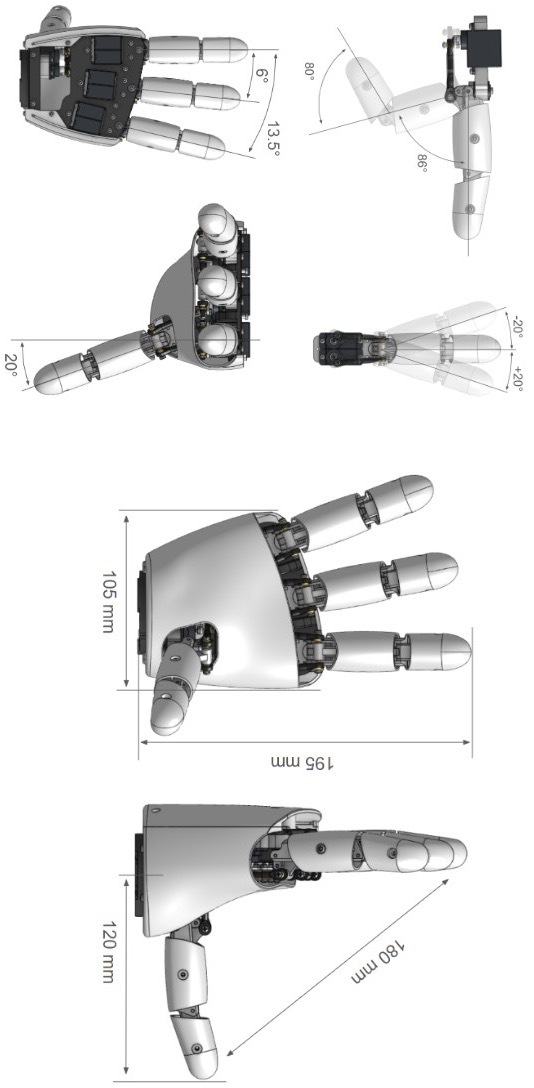
\includegraphics[width=0.75\marginparwidth]{figures/amazinghand.jpg}\par}
\newthought{Why TPU?} It is strong yet stays flexible after
printing. We first used it for a robotic skin on the AmazingHand by
Pollen Robotics, pictured above, making a gripper surface more adaptable
and raising grip success rates.}

\index{AMS}\newthought{TPU runs from the external spool holder.} TPU never goes through the AMS. The flexible filament coils
inside the AMS hub instead of advancing down its Bowden path. You don't want to spend the time cleaning this.
So this is a mishap to avoid and not to experience first-hand for a deeper learning experience. 
Because we can not use the AMS, we have to feed TPU directly into the extruder. 
This is a hands-on procedure that requires some care and attention.

\index{unloading filament}\newthought{unloading pla}
\begin{enumerate}[itemsep=2pt]
  \item On the printer screen open the gear \icongear{}, then
        \texttt{Filament}, and unload whatever is currently sitting in the
        extruder.
  \item Detach the tube on the back that runs from the AMS into the toolhead and
        park it clear of the feed path.
\end{enumerate}

\index{loading filament}\newthought{loading tpu}
\begin{enumerate}[itemsep=2pt]
  \item Hang the TPU spool on the external holder at the back of the
        printer (looks like a metal bar) and thread the loose end into the
        tube inlet the AMS tube used to occupy.
  \item On the printer screen choose the nozzle \iconnozzle{} icon, then
        \texttt{Feeding}, choose \texttt{Load}. While the printer runs the load, push the
        filament slightly in by hand until the feed gears grab it and
        take over. Watch the nozzle purge until a clean strand of TPU comes out. 
  \item In Bambu Studio open the \texttt{Device} tab. Next to the four
        AMS slots sits an \texttt{Ext} slot\index{Ext slot} for the external spool; select
        that one and set the filament type to \texttt{TPU}. 
\end{enumerate}


\marginnote{\newthought{One object per plate for a nicer result.} TPU's elasticity stretches into a hair
that drifts and tangles with movement between objects while printing. This messes up your surface and print quality.}

\index{stringing}\newthought{You are ready to print TPU.}  

\index{drying}\newthought{unloading tpu}
\marginnote{\newthought{Keep the spool dry.} TPU is hygroscopic. Off the
holder, store the spool in a sealed box with desiccant. A spool left in
open room air for a few days prints visibly worse.}
\begin{enumerate}[itemsep=2pt]
  \item On the printer screen choose the nozzle \iconnozzle{} icon, then
        \texttt{Feeding}, choose \texttt{Unload}. The printer heats the
        nozzle and retracts the filament.
  \item Once the feed gears release it,
  pull the strand back out of the tube inlet by hand and wind it
  onto the spool. Stow away TPU in a sealed box immediately.
\end{enumerate}

\newthought{loading pla again}
\begin{enumerate}[itemsep=2pt]
  \item Reattach the AMS tube you parked earlier to the tube inlet on the
        toolhead and push it in until it seats.
  \item On the printer screen open the gear \icongear{}, then
        \texttt{Filament}, select the AMS slot holding your PLA, and
        choose \texttt{Load}. The AMS feeds the filament down the Bowden
        path on its own; watch the nozzle purge until a clean strand of
        PLA comes out.
  \item In Bambu Studio open the \texttt{Device} tab and select the AMS
        slot instead of the \texttt{Ext} slot, so the next job pulls from
        the AMS again.
\end{enumerate}






% % !TEX root = ../notes_3dprinting.tex
% Chapter 2: Access and House Rules -- STUB
%%%%%%%%%%%%%%%%%%%%%%%%%%%%%%%%%%%%%%%%%%%%%%%%%%%%%%%%%%%%%%%%%%%%%%

\index{house rules}\index{Bambu account}
\chapter{Access and House Rules}
\printchapterversion{02_access}
\newthought{Before You Touch It.}

\newthought{To be written.} Bambu account and printer binding, the
\texttt{2.4~GHz} network constraint, safety in a shared room, and the rules of a
machine nobody owns alone.

% Planned sections, uncomment and fill:
% \section{Who prints, and the rules of a shared machine}
% \section{Safety: ABS fumes and the closed door, hot end, unattended prints}
% \section{Accounts: binding, the "already bound" failure, unbinding, sharing}
% \section{Network: 2.4 GHz only, and what that means on a campus network}
% \section{Bambu Studio versus Handy}

% % !TEX root = ../notes_3dprinting.tex
% Chapter 3: Anatomy of the Machine -- STUB
%%%%%%%%%%%%%%%%%%%%%%%%%%%%%%%%%%%%%%%%%%%%%%%%%%%%%%%%%%%%%%%%%%%%%%

\index{toolhead}\index{build plate}\index{AMS}
\chapter{Anatomy of the Machine}
\printchapterversion{03_anatomy}
\newthought{What Moves, What Melts.}

\newthought{To be written.} What the toolhead, the filament path, the AMS, and
the plate are, in the detail needed to reason about a failure.

% Planned sections, uncomment and fill:
% \section{CoreXY and the enclosure}
% \section{Toolhead: direct drive extruder, hotend, nozzle size and hardness}
% \section{The filament path: the AMS pushes, the external spool is pulled}
%   -> TikZ figure: both paths side by side. Carries most of the Materials chapter.
% \section{AMS and AMS 2 Pro: slot mapping, active drying, the P1 power adapter}
% \section{The textured PEI plate and what sticks to it}

% % !TEX root = ../notes_3dprinting.tex
% Chapter 4: Slicer Parameters -- STUB
%%%%%%%%%%%%%%%%%%%%%%%%%%%%%%%%%%%%%%%%%%%%%%%%%%%%%%%%%%%%%%%%%%%%%%

\index{slicing}\index{infill}\index{supports}
\chapter{Slicer Parameters}
\printchapterversion{04_slicer}
\newthought{The Knobs That Matter.}

\newthought{To be written.} The settings that change the part, and the ones that
only change the number in the corner of the screen.

% Planned sections, uncomment and fill:
% \section{Layer height}
% \section{Walls and shells: where strength actually comes from}
% \section{Infill: density, pattern, and when it does nothing}
% \section{Temperature, flow ratio, and the volumetric speed ceiling}
% \section{Cooling}
% \section{Speed, and what to give up first}
% \section{Supports: normal versus tree, interface layers}
% \section{Adhesion: brim, raft, and the first layer}
%   -> Table: parameter, default, raise when, lower when

% % !TEX root = ../notes_3dprinting.tex
% Chapter 5: Designing for the Machine -- STUB
%%%%%%%%%%%%%%%%%%%%%%%%%%%%%%%%%%%%%%%%%%%%%%%%%%%%%%%%%%%%%%%%%%%%%%

\index{design for additive manufacturing}\index{overhang}\index{tolerance}
\chapter{Designing for the Machine}
\printchapterversion{05_design}
\newthought{Grown, Not Cut.}

\newthought{To be written.} Orientation, tolerance, and the structure you add to
a part for no reason other than that it is grown in layers.

% Planned sections, uncomment and fill:
% \section{Orientation is the first decision}
% \section{Overhangs, bridges, and the 45 degree rule}
% \section{Dimensional truth: shrinkage, elephant foot, hole undersize, clearances}
% \section{Wall thickness as a multiple of extrusion width}
% \section{Stabilizing structure: brim, ribs, gussets, fillets, sacrificial towers}
%   -> Table: nominal feature, typical printed error, compensation

% % !TEX root = ../notes_3dprinting.tex
% Chapter 6: Materials -- WRITTEN
% Every number here was resolved from the local Bambu Studio profile tree,
% not from a datasheet or the wiki. Re-resolve before editing any of them.
%%%%%%%%%%%%%%%%%%%%%%%%%%%%%%%%%%%%%%%%%%%%%%%%%%%%%%%%%%%%%%%%%%%%%%

\index{PLA}\index{TPU}\index{ABS}\index{PETG-CF}
\chapter{Materials}
\printchapterversion{06_materials}
\newthought{What the Profiles Say.}

\newthought{The numbers below are not from a datasheet.} They are the resolved
values Bambu Studio itself loads for a P1S with a \texttt{0.4} nozzle on a
textured PEI plate, read out of the profile tree the application installs under
\texttt{system/BBL/filament/}. Those files are JSON with an \texttt{inherits}
chain, and resolving that chain gives the values a job actually runs with. When
the printer and this table disagree, the printer is right and this table is
stale.

\begin{table*}[ht]
\centering
\begin{tabular}{p{0.16\textwidth}p{0.14\textwidth}p{0.08\textwidth}p{0.15\textwidth}p{0.12\textwidth}p{0.19\textwidth}}
    \toprule
    \textbf{Material} & \textbf{Nozzle temp} & \textbf{Plate} & \textbf{Max flow} & \textbf{Hardness} & \textbf{Feed path} \\
    \midrule
    PLA Basic     & 220\,\textcelsius{}              & 55\,\textcelsius{} & 21\,mm\textsuperscript{3}/s   & any        & AMS \\[3pt]
    PETG-CF       & 255\,\textcelsius{}              & 70\,\textcelsius{} & 11.5\,mm\textsuperscript{3}/s & hardened   & AMS, dry it first \\[3pt]
    ABS           & 260, then 270\,\textcelsius{}    & 90\,\textcelsius{} & 16\,mm\textsuperscript{3}/s   & any        & AMS, door shut \\[3pt]
    TPU 95A HF    & 230\,\textcelsius{}              & 45\,\textcelsius{} & 12\,mm\textsuperscript{3}/s   & any        & external spool only \\[3pt]
    TPU 90A       & 225\,\textcelsius{}              & 35\,\textcelsius{} & 2.8\,mm\textsuperscript{3}/s  & any        & external spool only \\[3pt]
    TPU for AMS   & 230\,\textcelsius{}              & 35\,\textcelsius{} & 18\,mm\textsuperscript{3}/s   & any        & AMS \\
    \bottomrule
\end{tabular}
\vspace{2em}
\caption{Resolved P1S profile values, \texttt{0.4} nozzle, textured PEI plate.
ABS runs its first layer cooler than the rest. \textit{Max flow} is
\texttt{filament\_max\_volumetric\_speed}, the ceiling the slicer will not let
any speed setting exceed.}
\label{tab:materials}
\end{table*}

\newthought{Read the flow column, not the speed slider.} Volumetric flow is the
real throughput limit, and it is the only honest predictor of print time. TPU
90A at $2.8$\,mm\textsuperscript{3}/s moves roughly seven times less plastic per
second than PLA at $21$. Asking for 300\,mm/s changes nothing; the slicer simply
clamps the speed down to respect the ceiling.

\marginnote{\newthought{Why 85A is missing.} Its P1 series profile lists only the
$0.6$ and $0.8$ nozzles as compatible printers. With a $0.4$ installed, TPU 85A
is not an option on this machine.}

\newthought{TPU does not go in the AMS.} The AMS pushes filament down a long
Bowden path into the extruder, and a rigid filament transmits that push. A
flexible one compresses and coils inside the hub instead of advancing, and the
jam has to be dismantled by hand. This is a property of the feed direction, not
a firmware limit, so a second AMS unit does not change it. TPU goes on the
external spool holder at the back of the printer, where the extruder pulls it
over a short direct path.

\marginnote{\newthought{The one exception} is a distinct product, \texttt{Bambu
TPU for AMS}. It carries its own filament type, \texttt{TPU-AMS}, and is stiff
enough to survive being pushed. If the spool does not say so on the label, it is
standard TPU and belongs on the back.}

\newthought{PETG-CF needs a hardened nozzle.} Its profile demands a nozzle of
\texttt{HRC 40}; every other material listed here is happy with \texttt{HRC 3}.
Carbon fibre is abrasive and will open a soft $0.4$ orifice within a few hundred
grams of filament, after which every part prints over-extruded and nothing is
repeatable again.

\marginnote{\newthought{Filed under the wrong name.} PETG-CF has no profile
named for the P1S. It lives under \texttt{Bambu PETG-CF @BBL X1C} and lists the
P1S among its compatible printers. It is also hygroscopic enough that a spool
left open prints visibly worse within days.}

% % !TEX root = ../notes_3dprinting.tex
% Chapter 7: Sequenced Printing -- WRITTEN
% Pause mid print, drop a part into an open cavity, let the printer close
% over it. Not to be confused with print-by-object sequential printing.
%%%%%%%%%%%%%%%%%%%%%%%%%%%%%%%%%%%%%%%%%%%%%%%%%%%%%%%%%%%%%%%%%%%%%%

\index{pause}\index{inserts}\index{magnets}
\chapter{Sequenced Printing}
\printchapterversion{07_sequenced}
\newthought{Stop, Insert, Continue.}

\newthought{Some parts are best built in two sittings.} Print until a cavity is
open and reachable, stop, drop something into it, and let the printer close over
the top. The result is a captive part that could not be assembled afterwards:
a nut trapped in a pocket, a magnet buried flush, a bearing, a PCB, a cable
routed through a wall. Nothing about the machine is special here. The whole
technique is one pause in the right place.

\marginnote{\newthought{Not the same as sequential printing.} Bambu Studio also
offers printing several objects one after another, complete part by complete
part. That is a different feature with a different purpose. This chapter is
about pausing inside a single object.}

\newthought{The pause fires before its layer is printed.} That is the only
timing rule, and getting it backwards is the usual mistake. Scrub the preview
slider up until you find the first layer that closes over the cavity, the layer
where the hole disappears, and put the pause there. Bambu Studio emits a single
line of G-code at that point:

\begin{verbatim}
M400 U1     ; finish queued moves, then wait for me
\end{verbatim}

\newthought{Design the pocket loose, and deeper than the insert.} Give roughly
$0.1$ to $0.2$\,mm of clearance in plan so the insert drops in without force,
and the same again in depth so it sits below the surrounding surface. If the
insert stands proud by even one layer height, the nozzle will strike it on the
next pass. At best that knocks the insert out of place; at worst it shifts the
whole part off the plate and takes the print with it.

\newthought{The procedure, once the model is right:}

\begin{enumerate}[itemsep=2pt]
  \item Slice, then switch to the Preview tab.
  \item Drag the vertical layer slider up to the first layer that spans the
        cavity. Confirm on screen that the hole is gone at that layer and still
        open one layer below.
  \item Right-click the slider at that layer and choose \texttt{Add pause}.
  \item Send the job. The pause travels with the file, so re-slicing after a
        change means re-adding it.
  \item When the printer stops, the toolhead parks and the bed stays hot. Leave
        the plate exactly where it is. Do not lift it, do not rotate it.
  \item Seat the insert and press it flush. Check with a straight edge that
        nothing stands above the top surface.
  \item Resume from the printer screen or from Bambu Studio.
  \item Watch the first layer over the insert the same way you watch a first
        layer on the plate.
\end{enumerate}

\marginnote{\newthought{Have the insert in your hand} before the pause arrives.
The part cools while the printer waits. With PLA a minute costs nothing. With
ABS a long pause invites the layer below to contract and the bond across the
pause line to fail, which is exactly where the part will later break.}

\newthought{Two failure modes are specific to magnets.} Check the polarity
before it goes in, because it is not coming out again, and remember that a
magnet will happily reach through a thin floor and grab the steel plate. Leave
enough material underneath, or accept that removing the finished part becomes a
fight.

\marginnote{\newthought{Teaser.} If the pause fires before its layer is printed,
which layer do you select to bury a magnet whose pocket is $3$\,mm deep?}

% % !TEX root = ../notes_3dprinting.tex
% Chapter 8: Getting Geometry -- STUB
%%%%%%%%%%%%%%%%%%%%%%%%%%%%%%%%%%%%%%%%%%%%%%%%%%%%%%%%%%%%%%%%%%%%%%

\index{STL}\index{CAD}\index{3MF}
\chapter{Getting Geometry}
\printchapterversion{08_geometry}
\newthought{Where Models Come From.}

\newthought{To be written.} Where models come from, what you are licensed to do
with them, and which free CAD tool is worth the afternoon.

% Planned sections, uncomment and fill:
% \section{STL, STEP, and why you should ship 3MF}
% \section{Repositories: MakerWorld, Printables, Thingiverse, Thangs, GrabCAD}
% \section{Licences: what you may actually print and hand in}
% \section{Free CAD worth learning: Onshape, FreeCAD, OpenSCAD, Tinkercad}
% \section{Repairing a broken mesh}

% % !TEX root = ../notes_3dprinting.tex
% Chapter 9: Maintenance -- STUB
%%%%%%%%%%%%%%%%%%%%%%%%%%%%%%%%%%%%%%%%%%%%%%%%%%%%%%%%%%%%%%%%%%%%%%

\index{maintenance}\index{calibration}
\chapter{Maintenance}
\printchapterversion{09_maintenance}
\newthought{Before It Breaks.}

\newthought{To be written.} What to do at what interval, and which of it is
staff only.

% Planned sections, uncomment and fill:
% \section{The schedule, by interval}
% \section{The plate: the highest yield habit there is}
% \section{Motion: carbon rods are cleaned, lead screws are greased}
% \section{Extruder and hotend: wear, clogs, and the complete hot end swap}  % staff
% \section{The AMS: desiccant, PTFE, feeder gears}
% \section{Calibration: flow dynamics and vibration compensation}
% \section{Firmware}  % staff

% % !TEX root = ../notes_3dprinting.tex
% Chapter 10: Troubleshooting -- INTENTIONALLY EMPTY
% Grows from real failures on this machine. Do not pre-fill it with a
% generic catalogue; the outline below is a place to hang them, not a plan
% to execute.
%%%%%%%%%%%%%%%%%%%%%%%%%%%%%%%%%%%%%%%%%%%%%%%%%%%%%%%%%%%%%%%%%%%%%%

\index{troubleshooting}
\chapter{Troubleshooting}
\printchapterversion{10_troubleshooting}
\newthought{Filled by Failure.}

\newthought{Empty on purpose.} This chapter grows from real failures on this
machine rather than from a list of everything that could go wrong elsewhere.
When a print fails and you work out why, write it down here.

% Planned sections, uncomment and fill as failures actually occur:
% \section{Diagnose by reading the layer it failed on}
% \section{Filament snapped or ran out: the AMS case and the external case}
%   -> numbered procedure, the one place enumerate is justified
% \section{Clogs and no extrusion}
% \section{First layer failures}
% \section{Spaghetti, layer shift, aborted prints}
% \section{AMS faults}
% \section{Triage table: symptom, first check, fix}


% Register the vendor documentation so the reference machinery has entries to
% resolve even while most chapters are still stubs.
\nocite{bambulab2026wiki,bambulab2026hotend,bambulab2026tpu}
\makestandardbackmatter{printing}

\end{document}
